% The cubic y^2=x^3-x+1 with the line through P, Q, R and the vertical line through R. Generated by a short script.
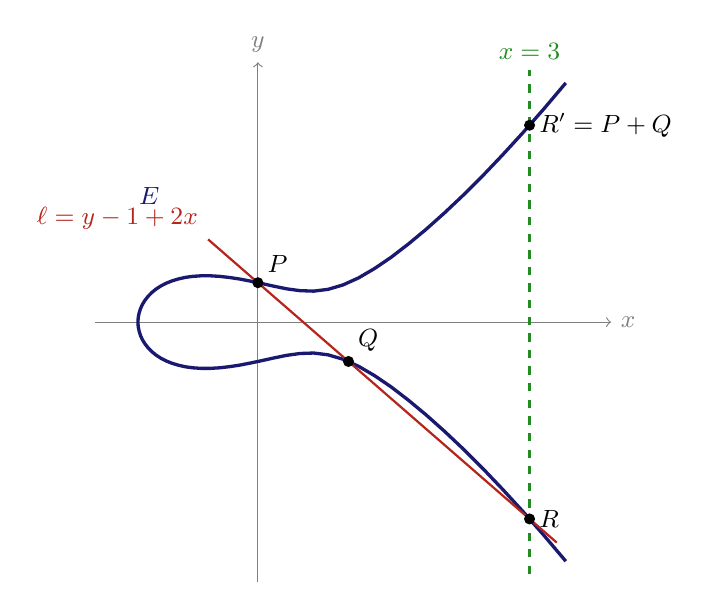
\begin{tikzpicture}[font=\small,x=1.15cm,y=1cm]
\draw[->,gray] (-1.8,0) -- (3.9,0) node[right] {$x$};
\draw[->,gray] (0,-3.3) -- (0,3.3) node[above] {$y$};
\draw[very thick,MidnightBlue] (3.400,-3.037) -- (3.161,-2.712) -- (2.928,-2.407) -- (2.701,-2.122) -- (2.481,-1.856) -- (2.266,-1.610) -- (2.058,-1.384) -- (1.856,-1.177) -- (1.660,-0.990) -- (1.471,-0.823) -- (1.288,-0.680) -- (1.111,-0.561) -- (0.940,-0.472) -- (0.775,-0.416) -- (0.617,-0.393) -- (0.465,-0.399) -- (0.319,-0.422) -- (0.179,-0.455) -- (0.045,-0.489) -- (-0.082,-0.520) -- (-0.203,-0.547) -- (-0.318,-0.567) -- (-0.427,-0.581) -- (-0.529,-0.588) -- (-0.626,-0.588) -- (-0.716,-0.581) -- (-0.800,-0.568) -- (-0.877,-0.548) -- (-0.949,-0.523) -- (-1.014,-0.493) -- (-1.073,-0.458) -- (-1.126,-0.418) -- (-1.173,-0.374) -- (-1.213,-0.327) -- (-1.247,-0.277) -- (-1.275,-0.225) -- (-1.297,-0.170) -- (-1.312,-0.114) -- (-1.322,-0.057) -- (-1.325,-0.000) -- (-1.322,0.057) -- (-1.312,0.114) -- (-1.297,0.170) -- (-1.275,0.225) -- (-1.247,0.277) -- (-1.213,0.327) -- (-1.173,0.374) -- (-1.126,0.418) -- (-1.073,0.458) -- (-1.014,0.493) -- (-0.949,0.523) -- (-0.877,0.548) -- (-0.800,0.568) -- (-0.716,0.581) -- (-0.626,0.588) -- (-0.529,0.588) -- (-0.427,0.581) -- (-0.318,0.567) -- (-0.203,0.547) -- (-0.082,0.520) -- (0.045,0.489) -- (0.179,0.455) -- (0.319,0.422) -- (0.465,0.399) -- (0.617,0.393) -- (0.775,0.416) -- (0.940,0.472) -- (1.111,0.561) -- (1.288,0.680) -- (1.471,0.823) -- (1.660,0.990) -- (1.856,1.177) -- (2.058,1.384) -- (2.266,1.610) -- (2.481,1.856) -- (2.701,2.122) -- (2.928,2.407) -- (3.161,2.712) -- (3.400,3.037);
\draw[thick,BrickRed] (-0.55,{0.5*(1-2*(-0.55))}) node[above left] {$\ell=y-1+2x$} -- (3.3,{0.5*(1-2*3.3)});
\draw[thick,dashed,ForestGreen] (3,-3.2) -- (3,3.2) node[above] {$x=3$};
\fill (0,0.5) circle (2pt) node[above right] {$P$};
\fill (1,-0.5) circle (2pt) node[above right] {$Q$};
\fill (3,-2.5) circle (2pt) node[right] {$R$};
\fill (3,2.5) circle (2pt) node[right] {$R'=P+Q$};
\node[MidnightBlue] at (-1.2,1.6) {$E$};
\end{tikzpicture}
